\chapter{平方根算法}

\index{square root algorithm}

\key{平方根算法}是指时间复杂度中含有平方根的算法。平方根可以看作“穷人的对数”：$O(\sqrt n)$ 优于 $O(n)$，但劣于 $O(\log n)$。无论如何，许多平方根算法在实践中速度很快，具有实用价值。

例如，考虑建立一种支持两种数组操作的数据结构：修改指定位置的元素，以及计算给定区间的元素和。此前我们用树状数组和线段树解决过该问题，两种操作的时间复杂度均为 $O(\log n)$。这里采用另一种平方根结构，使单点修改只需 $O(1)$ 时间，区间求和只需 $O(\sqrt n)$ 时间。

其思想是把数组划分成大小为 $\sqrt n$ 的若干\emph{块}，每个块存储块内元素之和。例如，一个包含 16 个元素的数组可按如下方式划分为每块 4 个元素：

\begin{center}
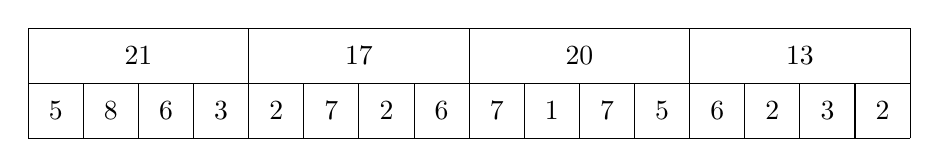
\begin{tikzpicture}[scale=0.7]
\draw (0,0) grid (16,1);

\draw (0,1) rectangle (4,2);
\draw (4,1) rectangle (8,2);
\draw (8,1) rectangle (12,2);
\draw (12,1) rectangle (16,2);

\node at (0.5, 0.5) {5};
\node at (1.5, 0.5) {8};
\node at (2.5, 0.5) {6};
\node at (3.5, 0.5) {3};
\node at (4.5, 0.5) {2};
\node at (5.5, 0.5) {7};
\node at (6.5, 0.5) {2};
\node at (7.5, 0.5) {6};
\node at (8.5, 0.5) {7};
\node at (9.5, 0.5) {1};
\node at (10.5, 0.5) {7};
\node at (11.5, 0.5) {5};
\node at (12.5, 0.5) {6};
\node at (13.5, 0.5) {2};
\node at (14.5, 0.5) {3};
\node at (15.5, 0.5) {2};

\node at (2, 1.5) {21};
\node at (6, 1.5) {17};
\node at (10, 1.5) {20};
\node at (14, 1.5) {13};

\end{tikzpicture}
\end{center}

在这种结构中，修改数组元素很容易：每次修改后只需更新一个块的元素和，时间复杂度为 $O(1)$。例如，下图展示了某个元素的值及其所在块的元素和如何变化：

\begin{center}
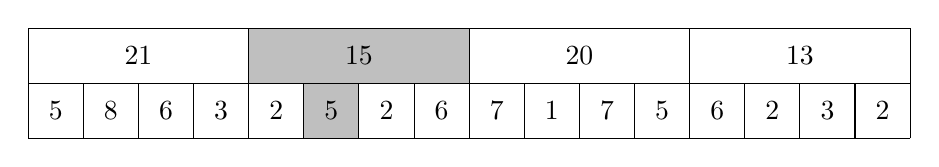
\begin{tikzpicture}[scale=0.7]
\fill[color=lightgray] (5,0) rectangle (6,1);
\draw (0,0) grid (16,1);

\fill[color=lightgray] (4,1) rectangle (8,2);
\draw (0,1) rectangle (4,2);
\draw (4,1) rectangle (8,2);
\draw (8,1) rectangle (12,2);
\draw (12,1) rectangle (16,2);

\node at (0.5, 0.5) {5};
\node at (1.5, 0.5) {8};
\node at (2.5, 0.5) {6};
\node at (3.5, 0.5) {3};
\node at (4.5, 0.5) {2};
\node at (5.5, 0.5) {5};
\node at (6.5, 0.5) {2};
\node at (7.5, 0.5) {6};
\node at (8.5, 0.5) {7};
\node at (9.5, 0.5) {1};
\node at (10.5, 0.5) {7};
\node at (11.5, 0.5) {5};
\node at (12.5, 0.5) {6};
\node at (13.5, 0.5) {2};
\node at (14.5, 0.5) {3};
\node at (15.5, 0.5) {2};

\node at (2, 1.5) {21};
\node at (6, 1.5) {15};
\node at (10, 1.5) {20};
\node at (14, 1.5) {13};

\end{tikzpicture}
\end{center}

计算一个区间的元素和时，把区间分为三部分，使答案由两端的单个元素以及中间若干整块的元素和组成：

\begin{center}
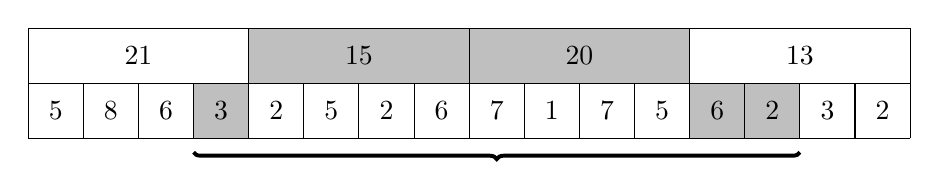
\begin{tikzpicture}[scale=0.7]
\fill[color=lightgray] (3,0) rectangle (4,1);
\fill[color=lightgray] (12,0) rectangle (13,1);
\fill[color=lightgray] (13,0) rectangle (14,1);
\draw (0,0) grid (16,1);

\fill[color=lightgray] (4,1) rectangle (8,2);
\fill[color=lightgray] (8,1) rectangle (12,2);
\draw (0,1) rectangle (4,2);
\draw (4,1) rectangle (8,2);
\draw (8,1) rectangle (12,2);
\draw (12,1) rectangle (16,2);

\node at (0.5, 0.5) {5};
\node at (1.5, 0.5) {8};
\node at (2.5, 0.5) {6};
\node at (3.5, 0.5) {3};
\node at (4.5, 0.5) {2};
\node at (5.5, 0.5) {5};
\node at (6.5, 0.5) {2};
\node at (7.5, 0.5) {6};
\node at (8.5, 0.5) {7};
\node at (9.5, 0.5) {1};
\node at (10.5, 0.5) {7};
\node at (11.5, 0.5) {5};
\node at (12.5, 0.5) {6};
\node at (13.5, 0.5) {2};
\node at (14.5, 0.5) {3};
\node at (15.5, 0.5) {2};

\node at (2, 1.5) {21};
\node at (6, 1.5) {15};
\node at (10, 1.5) {20};
\node at (14, 1.5) {13};

\draw [decoration={brace}, decorate, line width=0.5mm] (14,-0.25) -- (3,-0.25);

\end{tikzpicture}
\end{center}

由于单个元素的数量为 $O(\sqrt n)$，整块的数量也为 $O(\sqrt n)$，所以求和查询只需 $O(\sqrt n)$ 时间。把块大小设为 $\sqrt n$，是为了在两个量之间取得\emph{平衡}：数组被分成 $\sqrt n$ 个块，每块包含 $\sqrt n$ 个元素。

实践中不必严格取 $\sqrt n$，也可以使用 $k$ 和 $n/k$ 作为参数，其中 $k$ 与 $\sqrt n$ 不同。最优参数取决于具体问题和输入。例如，若算法经常遍历块、却很少检查块内的单个元素，则可以把数组分成 $k < \sqrt n$ 个块，每块包含 $n/k > \sqrt n$ 个元素。

\section{组合算法}

本节讨论两种把两个算法组合起来的平方根算法。在两种情形中，单独使用任意一种算法都能以 $O(n^2)$ 时间解决问题；而将二者结合后，运行时间只有 $O(n \sqrt n)$。

\subsubsection{分类处理}

假设给定一个包含 $n$ 个单元格的二维网格，每个单元格中都有一个字母。任务是找出字母相同且距离最小的两个单元格，其中 $(x_1,y_1)$ 与 $(x_2,y_2)$ 之间的距离为 $|x_1-x_2|+|y_1-y_2|$。例如，考虑下面的网格：

\begin{center}
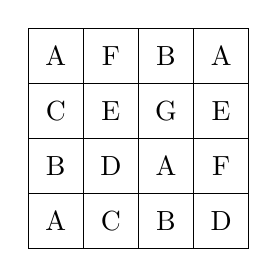
\begin{tikzpicture}[scale=0.7]
\node at (0.5,0.5) {A};
\node at (0.5,1.5) {B};
\node at (0.5,2.5) {C};
\node at (0.5,3.5) {A};
\node at (1.5,0.5) {C};
\node at (1.5,1.5) {D};
\node at (1.5,2.5) {E};
\node at (1.5,3.5) {F};
\node at (2.5,0.5) {B};
\node at (2.5,1.5) {A};
\node at (2.5,2.5) {G};
\node at (2.5,3.5) {B};
\node at (3.5,0.5) {D};
\node at (3.5,1.5) {F};
\node at (3.5,2.5) {E};
\node at (3.5,3.5) {A};
\draw (0,0) grid (4,4);
\end{tikzpicture}
\end{center}
此例中，两个字母 E 之间的最小距离为 2。

可以分别考虑每个字母来解决问题。这样，问题变成：对一个\emph{固定}字母 $c$，计算两个含有该字母的单元格之间的最小距离。考虑以下两种算法：

\emph{算法 1：}遍历所有包含字母 $c$ 的单元格对，计算它们之间的最小距离。若字母 $c$ 出现于 $k$ 个单元格中，时间复杂度为 $O(k^2)$。

\emph{算法 2：}从所有包含字母 $c$ 的单元格同时开始广度优先搜索，在 $O(n)$ 时间内求出两个此类单元格之间的最小距离。

一种解法是选择其中一种算法，并用于所有字母。若使用算法 1，运行时间为 $O(n^2)$，因为所有单元格可能都含有同一个字母，此时 $k=n$。若使用算法 2，运行时间同样为 $O(n^2)$，因为所有单元格可能含有不同字母，此时需要进行 $n$ 次搜索。

不过，可以\emph{组合}这两种算法，根据每个字母在网格中的出现次数选用不同算法。假设字母 $c$ 出现 $k$ 次：若 $k \le \sqrt n$，使用算法 1；若 $k > \sqrt n$，使用算法 2。这样做后，总运行时间只有 $O(n \sqrt n)$。

首先，假设对字母 $c$ 使用算法 1。由于 $c$ 在网格中至多出现 $\sqrt n$ 次，每个含有 $c$ 的单元格只需与其他单元格比较 $O(\sqrt n)$ 次，因此处理所有这类单元格共需 $O(n \sqrt n)$ 时间。再假设对字母 $c$ 使用算法 2。满足条件的字母至多有 $\sqrt n$ 个，所以处理这些字母同样只需 $O(n \sqrt n)$ 时间。

\subsubsection{分批处理}

下一个问题同样涉及一个包含 $n$ 个单元格的二维网格。初始时，除一个单元格外其余全部为白色。进行 $n-1$ 次操作，每次先计算某个给定白色单元格到黑色单元格的最短距离，再把该白色单元格染成黑色。

例如，考虑下面这次操作：

\begin{center}
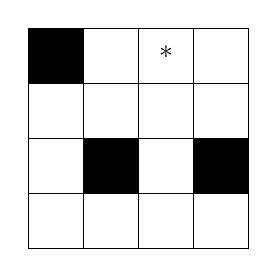
\begin{tikzpicture}[scale=0.7]
\fill[color=black] (1,1) rectangle (2,2);
\fill[color=black] (3,1) rectangle (4,2);
\fill[color=black] (0,3) rectangle (1,4);
\node at (2.5,3.5) {*};
\draw (0,0) grid (4,4);
\end{tikzpicture}
\end{center}

首先，计算标有 * 的白色单元格到黑色单元格的最短距离。向左移动两步即可到达黑色单元格，所以最短距离为 2。随后把该白色单元格染成黑色：

\begin{center}
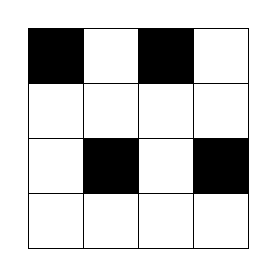
\begin{tikzpicture}[scale=0.7]
\fill[color=black] (1,1) rectangle (2,2);
\fill[color=black] (3,1) rectangle (4,2);
\fill[color=black] (0,3) rectangle (1,4);
\fill[color=black] (2,3) rectangle (3,4);
\draw (0,0) grid (4,4);
\end{tikzpicture}
\end{center}

考虑以下两种算法：

\emph{算法 1：}使用广度优先搜索，计算每个白色单元格到最近黑色单元格的距离。这需要 $O(n)$ 时间；搜索完成后，可以在 $O(1)$ 时间内查询任意白色单元格到黑色单元格的最短距离。

\emph{算法 2：}维护一个已经染黑的单元格列表。每次操作时遍历该列表，再把新的单元格加入列表。若列表长度为 $k$，一次操作需要 $O(k)$ 时间。

把所有操作划分为 $O(\sqrt n)$ 个\emph{批次}，每个批次包含 $O(\sqrt n)$ 次操作，从而组合上述算法。每个批次开始时执行算法 1；随后用算法 2 处理该批次中的操作。批次之间清空算法 2 的列表。每次操作中，到黑色单元格的最短距离取算法 1 与算法 2 所得距离中的较小值。

所得算法的时间复杂度为 $O(n \sqrt n)$。一方面，算法 1 执行 $O(\sqrt n)$ 次，每次搜索需要 $O(n)$ 时间；另一方面，在一个批次内使用算法 2 时，列表只含 $O(\sqrt n)$ 个单元格（批次之间会清空列表），所以每次操作需要 $O(\sqrt n)$ 时间。

\section{整数拆分}

一些平方根算法基于如下观察：若把正整数 $n$ 表示为若干正整数之和，其中\emph{互不相同}的数最多只有 $O(\sqrt n)$ 个。这是因为，要让和式包含尽可能多的不同数字，就应选择\emph{较小}的数。若选择 $1,2,\ldots,k$，所得总和为
\[\frac{k(k+1)}{2}.\]
因此，不同数字的最大数量为 $k = O(\sqrt n)$。下面讨论两个可利用这一观察高效解决的问题。

\subsubsection{背包}

假设给定一列总和为 $n$ 的整数重量，任务是找出由这些重量的任意子集能够组成的所有和。例如，重量为 $\{1,3,3\}$ 时，可能的和如下：

\begin{itemize}[noitemsep]
\item $0$（空集）
\item $1$
\item $3$
\item $1+3=4$
\item $3+3=6$
\item $1+3+3=7$
\end{itemize}

使用标准背包方法（见第 7.4 节），可以按如下方式解决：定义函数 $\texttt{possible}(x,k)$，若用前 $k$ 个重量能够组成和 $x$，其值为 1，否则为 0。由于重量总和为 $n$，重量个数至多为 $n$，利用动态规划可在 $O(n^2)$ 时间内计算函数的所有值。

不过，利用不同重量至多只有 $O(\sqrt n)$ 种这一事实，可以提高算法效率。把相同的重量分组，每组在 $O(n)$ 时间内处理，从而得到时间复杂度为 $O(n \sqrt n)$ 的算法。

具体做法是使用一个数组，记录由目前已经处理的各组重量能够组成的和。数组含有 $n$ 个元素：若能组成和 $k$，第 $k$ 个元素为 1，否则为 0。处理一组重量时，从左到右扫描数组，记录利用该组与之前各组能够新组成的和。

\subsubsection{字符串构造}

给定长度为 $n$ 的字符串 \texttt{s}，以及总长度为 $m$ 的字符串集合 $D$，考虑计算用 $D$ 中字符串拼接成 \texttt{s} 的方案数。例如，若 $\texttt{s}=\texttt{ABAB}$ 且 $D=\{\texttt{A},\texttt{B},\texttt{AB}\}$，共有 4 种方案：

\begin{itemize}[noitemsep]
\item $\texttt{A}+\texttt{B}+\texttt{A}+\texttt{B}$
\item $\texttt{AB}+\texttt{A}+\texttt{B}$
\item $\texttt{A}+\texttt{B}+\texttt{AB}$
\item $\texttt{AB}+\texttt{AB}$
\end{itemize}

可以使用动态规划解决该问题。令 $\texttt{count}(k)$ 表示用 $D$ 中字符串构造前缀 $\texttt{s}[0 \ldots k]$ 的方案数，则 $\texttt{count}(n-1)$ 就是答案；配合 Trie 结构，可以在 $O(n^2)$ 时间内解决问题。

进一步利用字符串哈希，以及 $D$ 中不同字符串长度至多有 $O(\sqrt m)$ 种这一事实，可以得到更高效的解法。首先构造集合 $H$，存入 $D$ 中所有字符串的哈希值。随后计算 $\texttt{count}(k)$ 时，遍历所有满足“$D$ 中存在长度为 $p$ 的字符串”的 $p$，计算 $\texttt{s}[k-p+1 \ldots k]$ 的哈希值，并检查它是否属于 $H$。由于不同字符串长度至多有 $O(\sqrt m)$ 种，所得算法的运行时间为 $O(n \sqrt m)$。

\section{莫队算法}

\index{Mo's algorithm}

\key{莫队算法}\footnote{据文献 \cite{cod15} 所述，该算法以中国竞赛程序员莫涛命名，但这一技术更早已见于文献 \cite{ken06}。}适用于许多需要在\emph{静态}数组上处理区间查询的问题，即查询之间数组元素不发生变化。每次查询给出区间 $[a,b]$，要求根据位置 $a$ 到 $b$ 之间的数组元素计算某个值。由于数组是静态的，查询可以按任意顺序处理；莫队算法采用一种特殊顺序，以保证处理效率。

莫队算法维护数组的一个\emph{活动区间}，并始终掌握当前活动区间对应查询的答案。算法逐个处理查询，通过插入和删除元素来移动活动区间的两个端点。若数组包含 $n$ 个元素、共有 $n$ 次查询，且每次插入或删除元素需要 $O(f(n))$ 时间，则算法的时间复杂度为 $O(n \sqrt n f(n))$。

莫队算法的关键在于查询的处理顺序：把数组划分为大小为 $k=O(\sqrt n)$ 的块；若满足下列任一条件，查询 $[a_1,b_1]$ 就在查询 $[a_2,b_2]$ 之前处理：
\begin{itemize}
\item $\lfloor a_1/k \rfloor < \lfloor a_2/k \rfloor$ or
\item $\lfloor a_1/k \rfloor = \lfloor a_2/k \rfloor$ and $b_1 < b_2$.
\end{itemize}

因此，左端点位于同一块内的所有查询会连续处理，并按右端点排序。采用这种顺序，算法只会执行 $O(n \sqrt n)$ 次操作：左端点共移动 $O(n)$ 轮，每轮移动 $O(\sqrt n)$ 步；右端点共移动 $O(\sqrt n)$ 轮，每轮移动 $O(n)$ 步。因此，整个算法中两个端点合计移动 $O(n \sqrt n)$ 步。

\subsubsection*{示例}

例如，给定一组查询，每个查询对应数组中的一个区间，要求计算每个区间内\emph{不同}元素的数量。

莫队算法对查询的排序方式始终相同，但如何维护查询答案则取决于具体问题。在本问题中，可以维护数组 \texttt{count}，其中 $\texttt{count}[x]$ 表示元素 $x$ 在活动区间内出现的次数。

从一个查询转移到另一个查询时，活动区间会随之变化。例如，若当前区间为
\begin{center}
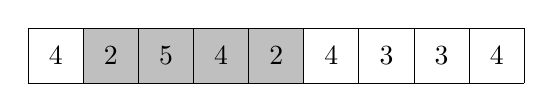
\begin{tikzpicture}[scale=0.7]
\fill[color=lightgray] (1,0) rectangle (5,1);
\draw (0,0) grid (9,1);
\node at (0.5, 0.5) {4};
\node at (1.5, 0.5) {2};
\node at (2.5, 0.5) {5};
\node at (3.5, 0.5) {4};
\node at (4.5, 0.5) {2};
\node at (5.5, 0.5) {4};
\node at (6.5, 0.5) {3};
\node at (7.5, 0.5) {3};
\node at (8.5, 0.5) {4};
\end{tikzpicture}
\end{center}
而下一个区间为
\begin{center}
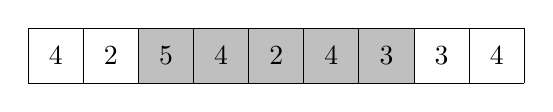
\begin{tikzpicture}[scale=0.7]
\fill[color=lightgray] (2,0) rectangle (7,1);
\draw (0,0) grid (9,1);
\node at (0.5, 0.5) {4};
\node at (1.5, 0.5) {2};
\node at (2.5, 0.5) {5};
\node at (3.5, 0.5) {4};
\node at (4.5, 0.5) {2};
\node at (5.5, 0.5) {4};
\node at (6.5, 0.5) {3};
\node at (7.5, 0.5) {3};
\node at (8.5, 0.5) {4};
\end{tikzpicture}
\end{center}
则需要三步：左端点向右移动一步，右端点向右移动两步。

每一步之后都要更新数组 \texttt{count}。加入元素 $x$ 后，把 $\texttt{count}[x]$ 加 1；若更新后 $\texttt{count}[x]=1$，查询答案也加 1。类似地，删除元素 $x$ 后，把 $\texttt{count}[x]$ 减 1；若更新后 $\texttt{count}[x]=0$，查询答案也减 1。

在本问题中，每一步操作只需 $O(1)$ 时间，所以算法的总时间复杂度为 $O(n \sqrt n)$。
